\documentclass[11pt]{article}

\usepackage[margin=1in]{geometry}
\usepackage[T1]{fontenc}
\usepackage{lmodern}
\usepackage{microtype}
\usepackage{amsmath,amssymb,amsthm,mathtools}
\usepackage[dvipsnames]{xcolor}
\usepackage[most]{tcolorbox}
\usepackage{tikz}
\usepackage{enumitem}
\usepackage{tocloft}
\usepackage[hidelinks]{hyperref}

\definecolor{courseblue}{HTML}{1F4E79}
\definecolor{lightblue}{HTML}{EAF2F8}
\definecolor{lightgreen}{HTML}{EAF7EA}
\definecolor{lightpink}{HTML}{FCE8EF}
\definecolor{darkgray}{HTML}{333333}

\setlength{\parindent}{0pt}
\setlength{\parskip}{0.65em}
\setlist[itemize]{topsep=0.25em,itemsep=0.15em}
\renewcommand{\cftsecleader}{\cftdotfill{\cftdotsep}}
\renewcommand{\cftsubsecleader}{\cftdotfill{\cftdotsep}}

\theoremstyle{plain}
\newtheorem{theorem}{Theorem}[section]
\newtheorem{proposition}[theorem]{Proposition}
\newtheorem{lemma}[theorem]{Lemma}
\theoremstyle{definition}
\newtheorem{definition}[theorem]{Definition}
\newtheorem{example}[theorem]{Example}
\newtheorem{exercise}[theorem]{Exercise}
\theoremstyle{remark}
\newtheorem*{remark}{Remark}

\tcolorboxenvironment{definition}{
  enhanced,
  colback=lightgreen,
  colframe=ForestGreen,
  boxrule=0.7pt,
  arc=2pt,
  left=6pt,
  right=6pt,
  top=5pt,
  bottom=5pt
}

\tcolorboxenvironment{exercise}{
  enhanced,
  colback=lightpink,
  colframe=WildStrawberry,
  boxrule=0.7pt,
  arc=2pt,
  left=6pt,
  right=6pt,
  top=5pt,
  bottom=5pt
}

\numberwithin{equation}{section}

\newcommand{\be}{\begin{eqnarray}}
\newcommand{\ee}{\end{eqnarray}}
\newcommand{\C}{\mathbb{C}}
\newcommand{\R}{\mathbb{R}}

\newcommand{\ww}{\mathbf w}
\newcommand{\hh}{\mathbf h}
\DeclareMathOperator{\Real}{Re}
\DeclareMathOperator{\Imag}{Im}
\tcbset{breakable}
\begin{document}

\begin{center}
  \colorbox{lightblue}{%
    \begin{minipage}{0.94\textwidth}
      \vspace{0.55em}
      \begin{tabular*}{\textwidth}{@{\extracolsep{\fill}}lr}
        {\color{courseblue}\bfseries\LARGE Lecture 4} &
        {\color{courseblue}\bfseries\LARGE MATH 411}\\[0.35em]
        \textbf{Fall 2026} & \textbf{Date: Sep 11, 2026}\\
        & \textbf{Instructor: Manish Patnaik}
      \end{tabular*}
      \vspace{0.45em}
    \end{minipage}}
\end{center}

\setcounter{tocdepth}{1}
\tableofcontents
\vspace{0.45em}



% Handwritten page 1.
\section{Review: complex differentiability and total differentiability}
\begin{definition}
Let $f:U\to\C$, where $U\subseteq\C$ is open. The function $f$ is
\emph{complex differentiable at $w\in U$} if
\be
 \lim_{h\to0}\frac{f(w+h)-f(w)}{h}
\ee
exists. This limit is denoted by $f'(w)$.

Equivalently, there exist a function $\sigma$ defined in a small
neighbourhood of $0\in\C$ and a complex number $\xi\in\C$ such that
\begin{enumerate}
\item $f(w+h)-f(w)-\xi h=\sigma(h)h$;
\item $\displaystyle\lim_{h\to0}\sigma(h)=0$.
\end{enumerate}
The neighbourhood is chosen small enough that $w+h\in U$.
In this formulation $\xi=f'(w)$.
\end{definition}

\begin{definition}
Now let $F$ be a function on an open set $U\subseteq\R^2$, with
\be
 F:U\to\R^2,\qquad
 \begin{pmatrix}x\\y\end{pmatrix}\longmapsto
 \begin{pmatrix}u(x,y)\\v(x,y)\end{pmatrix}.
\ee
The function $F$ is said to be \emph{totally differentiable} at the point
$\ww=\begin{pmatrix}x\\y\end{pmatrix}\in U$ if there exists a real $2\times2$ matrix
$D_{\ww}$ such that
\be
 \lim_{\|\hh\|\to0}
 \frac{F(\ww+\hh)-F(\ww)-D_{\ww}\hh}{\|\hh\|}
 =\begin{pmatrix}0\\0\end{pmatrix}.
\ee
Here $\hh$ is a vector in $\R^2$, and $\|\hh\|$ is its Euclidean norm.
\end{definition}

% Handwritten page 2.
\subsection*{Criterion from real analysis}
The existence of all four first partial derivatives alone does not imply
total differentiability, or even continuity.
\begin{example}
Define $F:\R^2\to\R^2$ by
\be
 F(x,y)=\begin{pmatrix}u(x,y)\\v(x,y)\end{pmatrix},\qquad
 u(x,y)=
 \begin{cases}
 \dfrac{x^2y}{x^4+y^2},&(x,y)\ne(0,0),\\[0.5em]
 0,&(x,y)=(0,0),
 \end{cases}
 \qquad v(x,y)=0.
\ee
Away from the origin, all four partial derivatives exist because the
defining functions are smooth. Since $u(t,0)=u(0,t)=0$ and $v=0$,
the difference quotients along the coordinate axes give
\be
 u_x(0,0)=u_y(0,0)=v_x(0,0)=v_y(0,0)=0.
\ee
Thus all four partial derivatives exist everywhere. However, along the
parabola $y=x^2$, for $t\ne0$ we have
\be
 u(t,t^2)=\frac{t^4}{t^4+t^4}=\frac12.
\ee
Consequently $F(t,t^2)=(\tfrac12,0)$ does not tend to $F(0,0)=(0,0)$
as $t\to0$. Thus $F$ is not continuous at the origin, and hence cannot
be totally differentiable there.

We can also check the definition directly. If $F$ were totally
differentiable at the origin, its derivative matrix
would have to be the zero matrix: applying the definition along each
coordinate axis forces both columns to vanish. But along
$\hh=(t,t^2)$, with $t\ne0$, we have
\be
 \frac{\|F(t,t^2)-F(0,0)\|}{\|(t,t^2)\|}
 =\frac{1}{2\sqrt{t^2+t^4}}
 \longrightarrow+\infty\qquad(t\to0).
\ee
This does not tend to zero. Hence $F$ is not totally differentiable at
$(0,0)$.
\end{example}

The following criterion gives a sufficient condition.
\begin{theorem}[Sufficient criterion for total differentiability]
\label{thm:total-differentiability-criterion}
If the first partial derivatives of $u$ and $v$ exist in a neighbourhood
of $\ww$ and are continuous at $\ww$, then $F$ is totally differentiable
at $\ww$, and its derivative matrix is the Jacobian
\be
 D_{\ww}=J_F(\ww)=
 \begin{pmatrix}u_x&u_y\\v_x&v_y\end{pmatrix}_{\ww}.
\ee
\end{theorem}
Note that continuity of the partial derivatives is a sufficient condition, but it is not a necessary condition for total
differentiability at a point. Total differentiability at $\ww$ does, however,
imply that all first partial derivatives exist at $\ww$ and form the matrix
$D_{\ww}$, even when those partial derivatives are not continuous there.

\section{The Cauchy--Riemann criterion}
What is the relation between total differentiability of $F$ and complex
differentiability of $f$? Identify $\C$ with $\R^2$ via
$x+iy\leftrightarrow(x,y)$, and let $U$ be open. Write
\be
 f:U\to\C,\qquad f(x+iy)=u(x,y)+iv(x,y),\qquad
 F(x,y)=\begin{pmatrix}u(x,y)\\v(x,y)\end{pmatrix}.
\ee
The naive guess is
\be
 F\text{ is totally differentiable at }\ww
 \quad\Longleftrightarrow\quad
 f\text{ is complex differentiable at }w.
\ee
This guess is false. The correct statement is the following.
\begin{theorem}
\label{thm:complex-differentiability-cr}
The function $f$ is complex differentiable at $w=x+iy$ if and only if
$F=\begin{pmatrix}u\\v\end{pmatrix}$ is totally differentiable at
$\ww=\begin{pmatrix}x\\y\end{pmatrix}$ and
\be
 \boxed{u_x=v_y,\qquad u_y=-v_x}
\ee
at $(x,y)$. These are the \emph{Cauchy--Riemann equations}.
\end{theorem}

\begin{remark}
In light of Theorem~\ref{thm:complex-differentiability-cr} and
Theorem~\ref{thm:total-differentiability-criterion}, we obtain the following
useful sufficient condition: $f$ is complex differentiable at $w=a+ib$
if $u_x,v_x,u_y,v_y$ all exist in a neighbourhood of $(a,b)$, are
continuous at $(a,b)$, and satisfy the Cauchy--Riemann equations
\be
 u_x(a,b)=v_y(a,b),\qquad u_y(a,b)=-v_x(a,b).
\ee
Equivalently, \emph{under the assumption that these partial derivatives
exist in a neighbourhood of $(a,b)$ and are continuous at $(a,b)$},
$f$ is complex differentiable at $a+ib$ if and only if the
Cauchy--Riemann equations hold there. Continuity of the partial derivatives,
together with the Cauchy--Riemann equations, is sufficient for complex
differentiability at a point; continuity of the partial derivatives is
not necessary.
\end{remark}

\section{Proof of the theorem}
We prove Theorem~\ref{thm:complex-differentiability-cr}. First suppose $f$ is complex differentiable at $w=x+iy$, and write
$f(x+iy)=u(x,y)+iv(x,y)$. We want to show that
\be
 F(x,y)=\begin{pmatrix}u(x,y)\\v(x,y)\end{pmatrix}
\ee
is totally differentiable at $\ww=(x,y)$ and that the Cauchy--Riemann
equations hold at $(x,y)$.

\subsection{Why is the associated real function totally differentiable?}
Since $f$ is complex differentiable, there exist a function $\sigma$ on
a neighbourhood of $0$ and a number $\alpha\in\C$ such that
\be
 f(w+h)-f(w)-\alpha h=\sigma(h)h,
 \qquad \lim_{h\to0}\sigma(h)=0.
\ee
Set
\be
 \ww=\begin{pmatrix}x\\y\end{pmatrix},\qquad
 \hh=\begin{pmatrix}r\\s\end{pmatrix},\qquad h=r+is.
\ee
Then
\be
 F(\ww+\hh)-F(\ww)=
 \begin{pmatrix}
 u(x+r,y+s)-u(x,y)\\
 v(x+r,y+s)-v(x,y)
 \end{pmatrix}.
\ee
We seek a matrix $D_{\ww}$ for which the components of
$F(\ww+\hh)-F(\ww)-D_{\ww}\hh$ are the real and imaginary parts of
\be
 f(w+h)-f(w)-\alpha h=\sigma(h)h.
\ee
% Handwritten page 4.
Write $\alpha=a+ib$. Since $h=r+is$, we have
\begin{align*}
 \alpha h&=(a+ib)(r+is)\\
 &=ar+ias+ibr+i^2bs\\
 &=(ar-bs)+i(as+br).
\end{align*}
The corresponding real matrix multiplication is
\be
 \begin{pmatrix}a&-b\\b&a\end{pmatrix}
 \begin{pmatrix}r\\s\end{pmatrix}
 =\begin{pmatrix}ar-bs\\as+br\end{pmatrix}.
\ee
Therefore choose
\be
 D_{\ww}=\begin{pmatrix}a&-b\\b&a\end{pmatrix}.
\ee
By what we have just observed,
\be{}
 F(\ww+\hh)-F(\ww)-D_{\ww}\hh
 =\begin{pmatrix}\Real(\sigma(h)h)\\\Imag(\sigma(h)h)\end{pmatrix}.
\ee Further, $\|\hh\|=\sqrt{r^2+s^2}=|h|$, so
\be
\begin{pmatrix}
	\Real\left(\dfrac{\sigma(h)h}{|h|}\right)\\[0.7em]
	\Imag\left(\dfrac{\sigma(h)h}{|h|}\right)
\end{pmatrix}
=\frac{F(\ww+\hh)-F(\ww)-D_{\ww}\hh}{\|\hh\|}.
\ee

By assumption, $\lim_{h\to0}\sigma(h)=0$, so we now need to consider
\be
 \lim_{h\to0}\frac{\sigma(h)h}{|h|}.
\ee
For $h\ne0$, write $h=|h|e^{i\theta_h}$. Thus
\be
 \frac{\sigma(h)h}{|h|}=\sigma(h)e^{i\theta_h}.
\ee
The number $e^{i\theta_h}$ lies on the unit circle. Consequently,
\be
 \left|\frac{\sigma(h)h}{|h|}\right|
 =|\sigma(h)|\,|e^{i\theta_h}|=|\sigma(h)|\longrightarrow0,
\ee
and hence
\be
 \lim_{h\to0}\frac{\sigma(h)h}{|h|}=0.
\ee
If this complex expression tends to zero, its real and imaginary parts
also tend to zero:
\be
 \Real\left(\frac{\sigma(h)h}{|h|}\right)\longrightarrow0,
 \qquad
 \Imag\left(\frac{\sigma(h)h}{|h|}\right)\longrightarrow0.
\ee

Both components tend to zero. This is exactly the definition of total
differentiability of $F$ at $\ww$.

% Handwritten page 5.
\subsection{Why do the Cauchy--Riemann equations hold?}
We now verify that the components $u$ and $v$ of the associated real
function satisfy the Cauchy--Riemann equations at the point under
consideration, $w=x+iy$. Write
\be
 f(w)=u(x,y)+iv(x,y).
\ee
\begin{center}
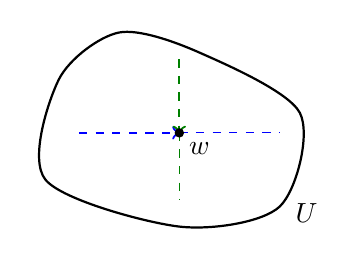
\begin{tikzpicture}[scale=0.85]
 \draw[thick] plot[smooth cycle] coordinates
 {(-2,-0.7) (-1.8,0.8) (-0.9,1.5) (0.3,1.2) (1.8,0.3) (1.5,-1.1) (0,-1.4)};
 \draw[blue,dashed,->,thick] (-1.5,0)--(0,0);
 \draw[blue,dashed] (0,0)--(1.5,0);
 \draw[green!50!black,dashed,->,thick] (0,1.1)--(0,0);
 \draw[green!50!black,dashed] (0,0)--(0,-1);
 \fill (0,0) circle (2pt);
 \node[below right] at (0,0) {$w$};
 \node at (1.9,-1.2) {$U$};
\end{tikzpicture}
\end{center}
First approach horizontally, so the complex increment is $h+i0$ with
$h\in\R$. Then
\begin{align*}
 f'(w)
 &=\lim_{\substack{h\to0\\h\in\R}}\frac{f(w+h)-f(w)}{h}\\
 &=\lim_{\substack{h\to0\\h\in\R}}
 \frac{u(x+h,y)+iv(x+h,y)-u(x,y)-iv(x,y)}{h}\\
 &=\lim_{\substack{h\to0\\h\in\R}}
 \frac{u(x+h,y)-u(x,y)}{h}
 +i\lim_{\substack{h\to0\\h\in\R}}
 \frac{v(x+h,y)-v(x,y)}{h}\\
 &=u_x(x,y)+iv_x(x,y).
\end{align*}
Thus
\be
 \boxed{f'(w)=u_x+iv_x.}
\ee
Next approach along the vertical axis. The complex increment is now $ih$,
where $h\in\R$. By the definition of the complex derivative, using this
vertical approach gives the same limit:
\be
 f'(w)=\lim_{\substack{h\to0\\h\in\R}}
 \frac{f(w+ih)-f(w)}{ih}.
\ee
% Handwritten page 6.
Expanding this expression yields
\begin{align*}
 f'(w)
 &=\lim_{\substack{h\to0\\h\in\R}}
 \frac{u(x,y+h)+iv(x,y+h)-u(x,y)-iv(x,y)}{ih}\\
 &=\lim_{\substack{h\to0\\h\in\R}}
 \frac{u(x,y+h)-u(x,y)}{ih}
 +\lim_{\substack{h\to0\\h\in\R}}
 \frac{i\bigl(v(x,y+h)-v(x,y)\bigr)}{ih}\\
 &=\frac1i\lim_{\substack{h\to0\\h\in\R}}
 \frac{u(x,y+h)-u(x,y)}{h}
 +\lim_{\substack{h\to0\\h\in\R}}
 \frac{v(x,y+h)-v(x,y)}{h}\\
 &=-iu_y(x,y)+v_y(x,y),\qquad\text{since }\frac1i=-i.
\end{align*}
Therefore
\be
 \boxed{f'(w)=-iu_y+v_y=u_x+iv_x.}
\ee
Equating real and imaginary parts gives
\be
 \boxed{u_x=v_y,\qquad v_x=-u_y.}
\ee
This proves the forward implication: complex differentiability of $f$
implies total differentiability of $F$ and the Cauchy--Riemann equations.
The reverse implication is proved next.

\subsection*{The reverse implication}

Suppose $F$ is totally differentiable at $\ww$ and the Cauchy--Riemann
equations hold there. All partial derivatives below are evaluated at
$(x,y)$. The derivative matrix is
\be
 D_{\ww}=\begin{pmatrix}u_x&u_y\\v_x&v_y\end{pmatrix}
 =\begin{pmatrix}a&-b\\b&a\end{pmatrix},
 \qquad a=u_x=v_y,\quad b=v_x=-u_y.
\ee
Set $\alpha=a+ib$ and let
\be
 E(\hh)=F(\ww+\hh)-F(\ww)-D_{\ww}\hh
 =\begin{pmatrix}E_1(\hh)\\E_2(\hh)\end{pmatrix}.
\ee
Total differentiability means $\|E(\hh)\|/\|\hh\|\to0$.
For $h=r+is$ corresponding to $\hh=\begin{pmatrix}r\\s\end{pmatrix}$, the matrix
calculation above gives
\be
 f(w+h)-f(w)-\alpha h=E_1(\hh)+iE_2(\hh).
\ee
For $h\ne0$, divide by $h$ and take absolute values:
\begin{align*}
 \left|\frac{f(w+h)-f(w)}h-\alpha\right|
 &=\frac{|E_1(\hh)+iE_2(\hh)|}{|h|}\\
 &=\frac{\sqrt{E_1(\hh)^2+E_2(\hh)^2}}{\|\hh\|}\\
 &=\frac{\|E(\hh)\|}{\|\hh\|}\longrightarrow0.
\end{align*}
Thus $f'(w)$ exists and equals $\alpha=u_x+iv_x$.

\section{Examples}
\subsection{The exponential function is entire}
Let $z=x+iy$. We show that $e^z$ is entire, that is, complex
differentiable at every point of $\C$. By
Theorems~\ref{thm:total-differentiability-criterion}
and~\ref{thm:complex-differentiability-cr}, it is sufficient to
verify that the first partial derivatives exist and are continuous, and
that $u$ and $v$ satisfy the Cauchy--Riemann equations.
\begin{align*}
 e^z&=e^x e^{iy}\\
 &=e^x\bigl(\cos y+i\sin y\bigr)\\
 &=\underbrace{e^x\cos y}_{u(x,y)}
   +i\underbrace{e^x\sin y}_{v(x,y)}.
\end{align*}
The four partial derivatives are
\begin{align*}
 u_x&=e^x\cos y,&v_x&=e^x\sin y,\\
 u_y&=-e^x\sin y,&v_y&=e^x\cos y.
\end{align*}
They exist and are continuous everywhere, and
\be
 u_x=v_y,\qquad u_y=-v_x.
\ee
The derivative matrix has precisely the indicated pattern:
\be
 J_F=\begin{pmatrix}
 e^x\cos y&-e^x\sin y\\
 e^x\sin y&e^x\cos y
 \end{pmatrix}.
\ee
Hence the theorem shows that $e^z$ is entire. The derivative formula also gives
\be
 (e^z)'=u_x+iv_x=e^x\cos y+ie^x\sin y=e^z.
\ee

% Handwritten page 7.
\begin{tcolorbox}[
 enhanced,breakable,
 colback=red!4,colframe=red!70!black,
 colbacktitle=red!70!black,coltitle=white,
 fonttitle=\bfseries,
 title={Warning: The Cauchy--Riemann equations alone do not suffice},
 boxrule=0.7pt,arc=2pt,
 left=6pt,right=6pt,top=5pt,bottom=5pt
]
Just because $u$ and $v$ satisfy the Cauchy--Riemann equations at a point
does not mean that $f(z)=u(x,y)+iv(x,y)$ is complex differentiable there. For example, let
\be
 f(z)=\begin{cases}
 \dfrac{z^5}{|z|^4},&z\ne0,\\[0.6em]
 0,&z=0.
 \end{cases}
\ee
This function is continuous at the origin, since $|f(z)|=|z|$.
It satisfies the Cauchy--Riemann equations there but is not complex
differentiable there.

\textit{Verification of the partial derivatives.} For real $t\ne0$, $|t|^4=t^4$ and $i^5=i$, so
\be
 f(t)=\frac{t^5}{|t|^4}=t,\qquad
 f(it)=\frac{i^5t^5}{|it|^4}=it.
\ee
Thus $u(t,0)=t$, $v(t,0)=0$, $u(0,t)=0$, $v(0,t)=t$, and
$u(0,0)=v(0,0)=0$. Consequently,
\begin{align*}
 u_x(0,0)&=\lim_{t\to0}\frac{u(t,0)-u(0,0)}t
 =\lim_{t\to0}\frac tt=1,\\
 v_x(0,0)&=\lim_{t\to0}\frac{v(t,0)-v(0,0)}t
 =\lim_{t\to0}\frac0t=0,\\
 u_y(0,0)&=\lim_{t\to0}\frac{u(0,t)-u(0,0)}t
 =\lim_{t\to0}\frac0t=0,\\
 v_y(0,0)&=\lim_{t\to0}\frac{v(0,t)-v(0,0)}t
 =\lim_{t\to0}\frac tt=1.
\end{align*}
Hence $u_x(0,0)=v_y(0,0)$ and $u_y(0,0)=-v_x(0,0)$.

For $h\ne0$, the difference quotient is
\begin{align*}
 \frac{f(0+h)-f(0)}h
 &=\frac{f(h)}h\\
 &=\frac{h^5/|h|^4}{h}\\
 &=\frac{h^4}{|h|^4}.
\end{align*}
Its limit as $h\to0$ does not exist. To see this explicitly, write
$h=re^{i\theta}$, where $r>0$. Then
\be
 \frac{h^4}{|h|^4}=\frac{r^4e^{4i\theta}}{r^4}=e^{4i\theta}.
\ee
Along the positive real axis ($\theta=0$), this quotient equals $1$.
Along the ray $\theta=\pi/4$, it equals $e^{i\pi}=-1$.
Both paths approach the origin as $r\to0$, but give different limits.
Therefore $f'(0)$ does not exist.
\end{tcolorbox}
%
%\subsection{Polar form of the Cauchy--Riemann equations}
%Suppose $f(z)=u(x,y)+iv(x,y)$ is written in polar coordinates, with
%$z=re^{i\theta}$ and $r>0$. Define the real-valued functions
%\be
% \widetilde u(r,\theta)=u(r\cos\theta,r\sin\theta),\qquad
% \widetilde v(r,\theta)=v(r\cos\theta,r\sin\theta).
%\ee
%Then
%\be
% f(re^{i\theta})=\widetilde u(r,\theta)+i\widetilde v(r,\theta).
%\ee
%Assume the Cartesian functions $u$ and $v$ are totally differentiable
%at the point in question, so that the chain rule applies. The
%Cauchy--Riemann equations take the polar form
%\be
% \boxed{\widetilde u_r=\frac1r\widetilde v_\theta,\qquad
% \frac1r\widetilde u_\theta=-\widetilde v_r.}
%\ee
%The tildes distinguish the polar functions from the Cartesian ones.
%
%\textit{Derivation.}
%Since $x=r\cos\theta$ and $y=r\sin\theta$, the chain rule gives
%\begin{align*}
% \widetilde u_r&=u_x\cos\theta+u_y\sin\theta,\\
% \widetilde v_r&=v_x\cos\theta+v_y\sin\theta,\\
% \widetilde u_\theta&=-r u_x\sin\theta+r u_y\cos\theta,\\
% \widetilde v_\theta&=-r v_x\sin\theta+r v_y\cos\theta.
%\end{align*}
%Here the Cartesian partial derivatives on the right are evaluated at
%$(x,y)=(r\cos\theta,r\sin\theta)$.
%Substituting $v_x=-u_y$ and $v_y=u_x$ yields
%\begin{align*}
% \frac1r\widetilde v_\theta
% &=-v_x\sin\theta+v_y\cos\theta\\
% &=u_y\sin\theta+u_x\cos\theta=\widetilde u_r,\\[0.3em]
% \frac1r\widetilde u_\theta
% &=-u_x\sin\theta+u_y\cos\theta\\
% &=-v_y\sin\theta-v_x\cos\theta=-\widetilde v_r.
%\end{align*}
%Conversely, set $A=u_x-v_y$ and $B=u_y+v_x$. The chain rule formulas
%show that the polar equations imply
%\be
% A\cos\theta+B\sin\theta=0,\qquad
% -A\sin\theta+B\cos\theta=0.
%\ee
%The coefficient matrix has determinant $\cos^2\theta+\sin^2\theta=1$,
%so $A=B=0$. Thus the Cartesian and polar Cauchy--Riemann equations
%are equivalent for $r>0$, under the total differentiability assumption.
\end{document}
